We evaluated \textbf{T1}-\textbf{T3} on Libsafe CVE-2005-1125 and on Libvirt CVE-2014-1447.
For each evaluation, exploit cost or exploit success rate was evaluated for each of many applications of the transformation under study.
The exploit cost or success rate was then compared to either the microbenchmark overhead, or the number of NOPs injected, as appropriate for each experiment.
Libsafe experiments were run on a dedicated dual core 3.4GHz Pentium D running Debian.
Libvirt experiments testing \textbf{T1} were run on a 2.7GHz dual-socket quad-core Intel Xeon with 16 hyper-threading cores running Debian.
Libvirt experiments testing \textbf{T2} and \textbf{T3} were run on a 2.8GHz dual-socket hex-core Intel Xeon with 24 hyper-threading cores running Ubuntu.
In all figures, the horizontal red line indicates the average measurement for the unmodified bug (without time randomization).
The results vary somewhat widely with the bug analyzed and the automated diversity transformation used.

Applying transformation 1
%(interposition of all external library function calls)
to Libsafe resulted in a dramatic decrease in exploit success rate with increasing microbenchmark overhead (Fig. \ref{fig_libsafe-all}).
Between 1x and 12x overhead, no randomizations resulted in less than a 5\% success rate.
Between 20x and 25x overhead, 27.5\% of randomizations resulted in less than a 5\% exploit success rate.
Between 40x and 45x overhead, 61.5\% of randomizations resulted in less than a 5\% exploit success rate.
Beyond 1,040x overhead, 100\% of randomizations resulted in less than a 5\% exploit success rate.
\begin{figure}
	\centering
	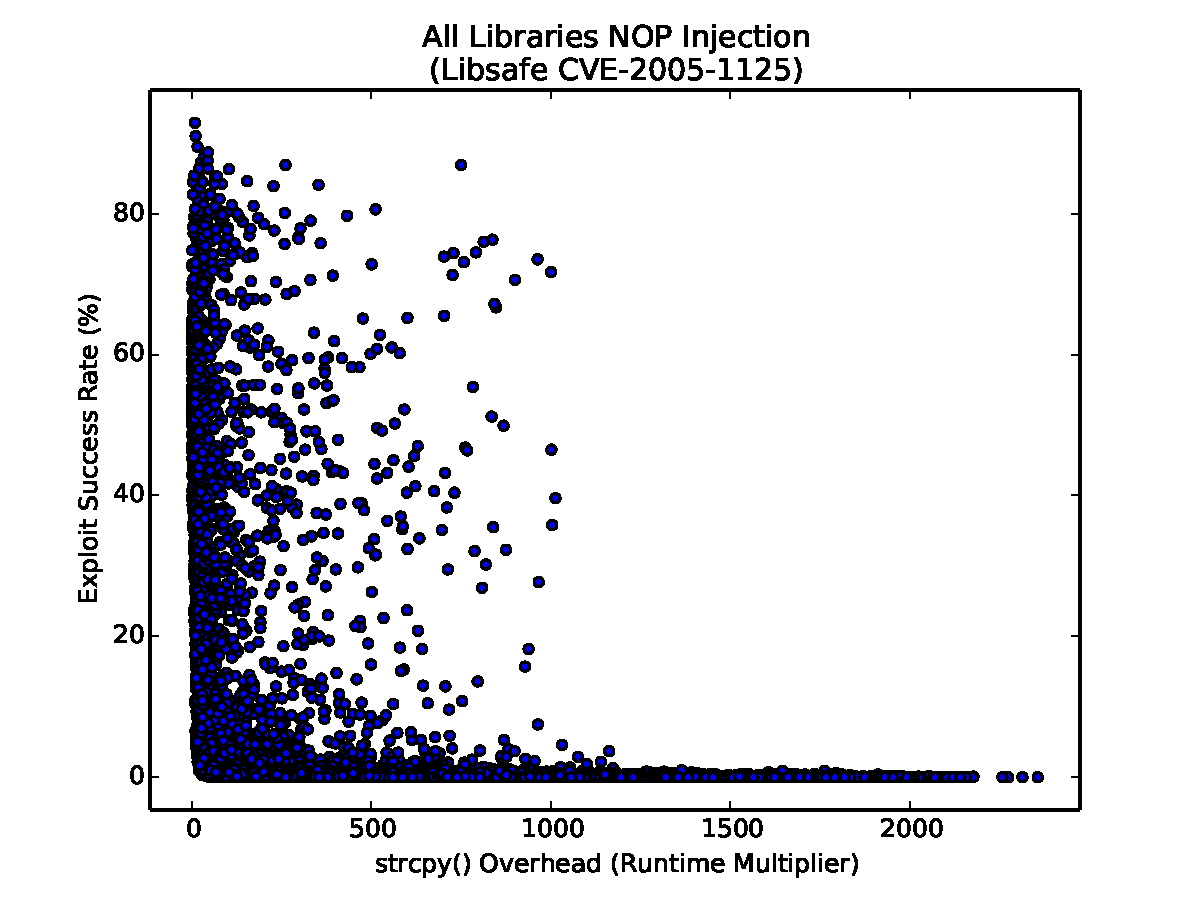
\includegraphics[width=.75\columnwidth]{figures/libsafe-all}
	\caption{Exploit success rate as a function of the microbenchmark after applying \textbf{T1} to Libsafe with concurrency bug CVE-2005-1125.
	There is a clear inverse correlation between microbenchmark overhead and exploit success rate.}
	\label{fig_libsafe-all}
\end{figure}

Applying \textbf{T2} to Libsafe had no noticeable effect on exploit success rate (Fig. \ref{fig_libsafe-pre}) or microbenchmark overhead.
\begin{figure}
	\centering
	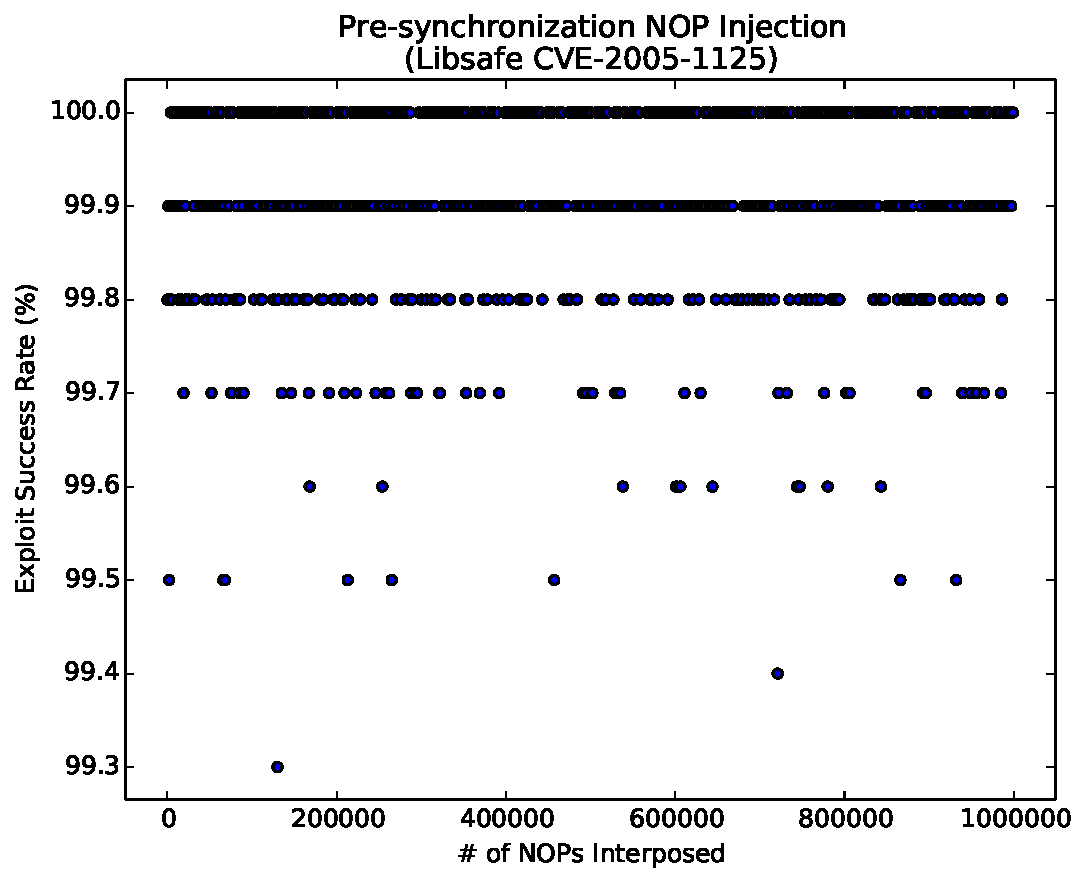
\includegraphics[width=.75\columnwidth]{figures/libsafe-pre}
	\caption{
		Exploit success rate as a function of the microbenchmark after applying diversity \textbf{T2} to Libsafe with concurrency bug CVE-2005-1125.
		This transformation does not appear to have an effect on exploit success rate for this bug.
	}
	\label{fig_libsafe-pre}
\end{figure}

Applying \textbf{T3} to Libsafe had a very marked effect on exploit success rate (Fig. \ref{fig_libsafe-post}).
In particular, the rate remains high for low numbers of NOPs.
Then, for inserted NOP loops of lengths greater than 200,000, the rate begins to drop.
For NOP loops of lengths between 250,000 and 350,000, exploit success rate fluctuates between 35\% and 65\%.
Finally, for NOP loops of lengths greater than 350,000, exploit rates drop even further, and beyond loop-lengths of 390,000 NOPs, all interpositions resulted in exploit rates less than 0.5\%.
\begin{figure}
	\centering
	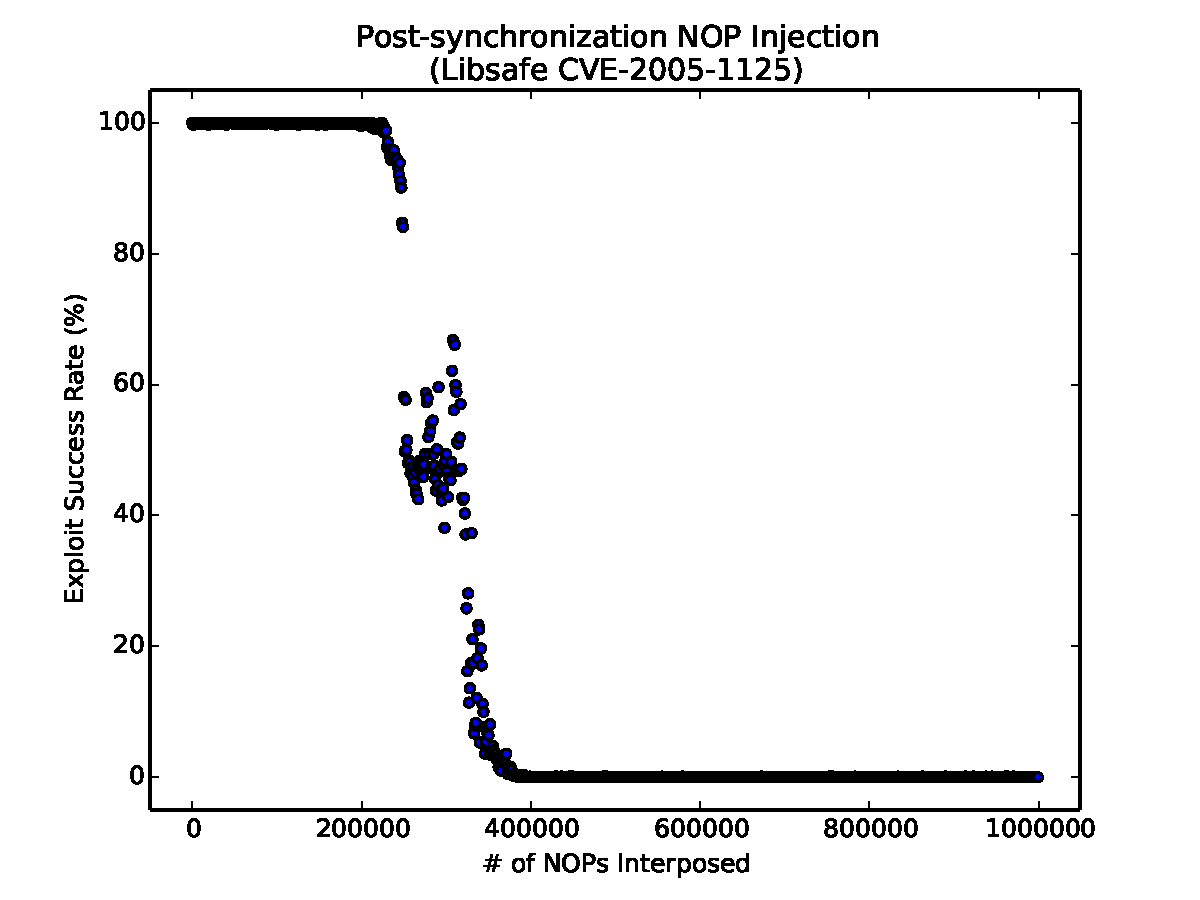
\includegraphics[width=.75\columnwidth]{figures/libsafe-post}
	\caption{
		Exploit success rate as a function of the number of NOPs injected after applying \textbf{T3} to Libsafe with concurrency bug CVE-2005-1125.
		A very clear inverse correlation between NOP loop length and exploit success rate is shown.
	}
	\label{fig_libsafe-post}
\end{figure}

\textbf{T1} affected the exploit cost for the Libvirt bug.
However, the increase in time required for exploitation is approximately proportional to the increase in microbenchmark measurements.
The exploit cost increase may therefore be attributed to an overall slowing down of the Libvirt daemon (Fig. \ref{fig_libvirt-all}).
\begin{figure}
	\centering
	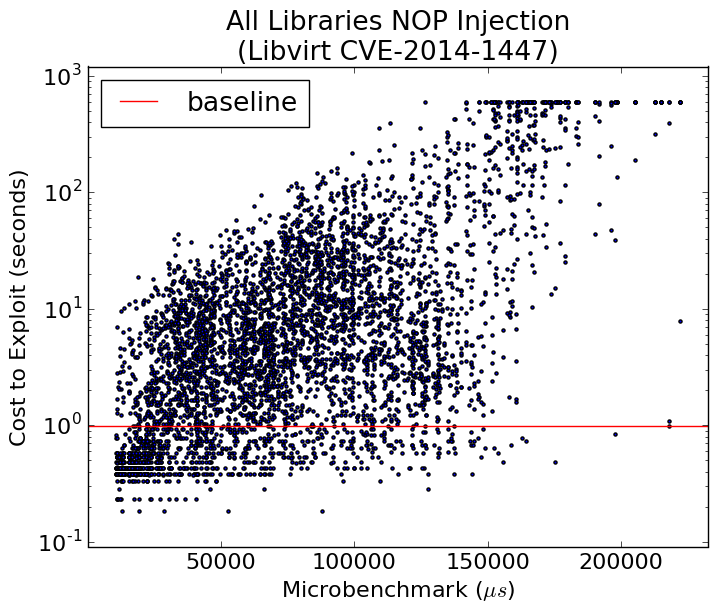
\includegraphics[width=.75\columnwidth]{figures/libvirt-all}
	\caption{
		Exploit cost (in time) as a function of the microbenchmark after applying \textbf{T1} to Libvirt with concurrency bug CVE-2014-1447.
		The exploit cost increases as a result of applying this transformation, but the increase is approximately proportional to the overall performance loss (x-axis).
	}
	\label{fig_libvirt-all}
\end{figure}

Applying \textbf{T2} to Libvirt did not seem to have much of an effect on exploit cost.
The characteristic of most exploit attempts succeeding quickly, and a few taking much longer appears to be consistent throughout the range of microbenchmark values recorded (Fig. \ref{fig_libvirt-pre}).
\begin{figure}
	\centering
	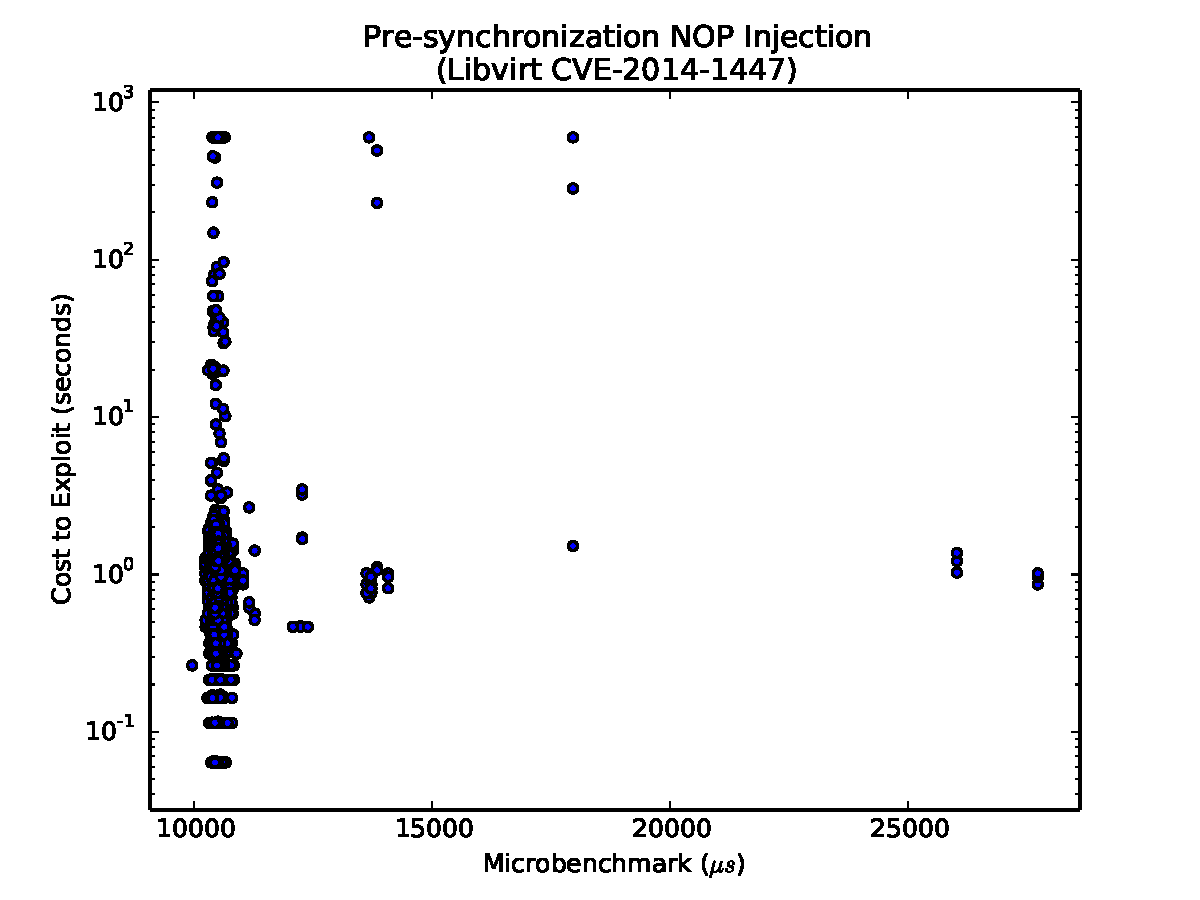
\includegraphics[width=.75\columnwidth]{figures/libvirt-pre}
	\caption{
		Exploit cost (in time) as a function of the microbenchmark after applying \textbf{T2} to Libvirt with concurrency bug CVE-2014-1447.
		This transformation does not appear to have an effect on exploit success rate for this bug.
	}
	\label{fig_libvirt-pre}
\end{figure}

\textbf{T3} applied to Libvirt, as in the case of Libsafe, had a significant effect on exploit cost.
For microbenchmark connection times of less than 10 milliseconds, less than 4\% of exploit attempts took longer than the baseline exploit time of 1.11 seconds, where the baseline exploit time was obtained for a Libvirt daemon without any time randomization.
By contrast, for microbenchmark times of greater than 10 milliseconds, nearly 85\% of exploit attempts took longer than the baseline exploit time.
Looking at the graph (Fig. \ref{fig_libvirt-post}), we can see a similar shape to the one obtained when applying \textbf{T2} to Libvirt - the bifurcation between exploit attempts that succeed quickly within seconds, and those which take hundreds of seconds to succeed.
However, after applying automated \textbf{T3}, a significantly greater proportion of exploit attempts fell into the second branch of that bifurcation, taking hundreds of seconds to succeed, or failing to succeed within ten minutes (and being categorized as failed attempts).
\begin{figure}
	\centering
	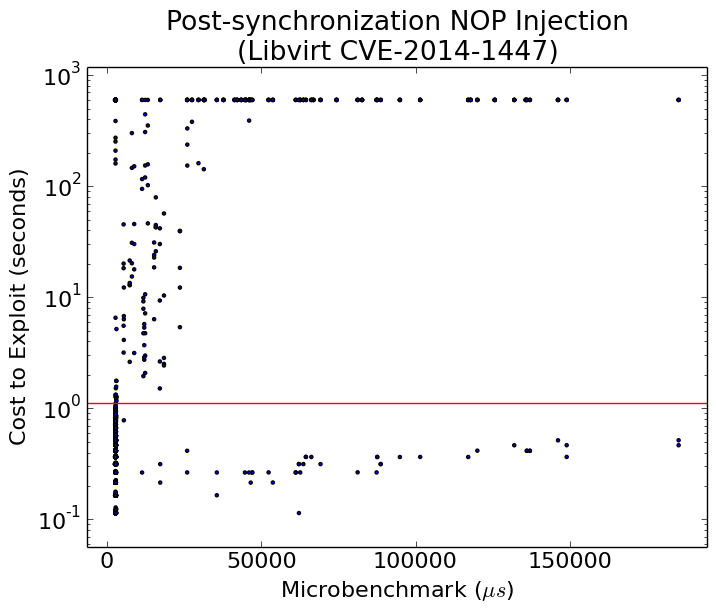
\includegraphics[width=.75\columnwidth]{figures/libvirt-post}
	\caption{
		Exploit cost (in time) as a function of the microbenchmark after applying diversity \textbf{T3} to Libvirt with concurrency bug CVE-2014-1447.
		Beyond microbenchmark measurements of 10 milliseconds, most of exploit costs observed were much greater than the baseline; often the exploit attempts were stopped artificially early and labeled ``failed exploits.''
		This transformation thus increases the average exploit cost with increasing microbenchmark overhead.
	}
	\label{fig_libvirt-post}
\end{figure}
